\documentclass[11pt,a4paper]{article}

% ---------- Packages ----------
\usepackage[utf8]{inputenc}
\usepackage[T1]{fontenc}
\usepackage[english]{babel}
\usepackage[a4paper,margin=2.5cm]{geometry}
\usepackage{amsmath,amssymb}
\usepackage{booktabs}
\usepackage{enumitem}
\usepackage{listings}
\usepackage{xcolor}
\usepackage{tikz}
\usetikzlibrary{arrows.meta,positioning}
\usepackage[hidelinks]{hyperref}
\emergencystretch=2em

% ---------- Code listing style ----------
\definecolor{lightgray}{gray}{0.95}
\definecolor{codegreen}{RGB}{0,110,50}
\definecolor{codeblue}{RGB}{20,40,160}
\lstdefinestyle{py}{
  language=Python,
  basicstyle=\ttfamily\footnotesize,
  keywordstyle=\color{codeblue}\bfseries,
  commentstyle=\color{codegreen}\itshape,
  stringstyle=\color{red!60!black},
  backgroundcolor=\color{lightgray},
  frame=single,
  rulecolor=\color{black!25},
  breaklines=true,
  showstringspaces=false,
  columns=fullflexible,
  xleftmargin=0.5em,
  xrightmargin=0.5em,
}
\lstset{style=py}

% ---------- Helper commands ----------
\newcommand{\alldiff}{\mathrm{alldifferent}}

% ---------- Title ----------
\title{\textbf{Generic Sudoku as a Constraint Satisfaction Problem}\\[0.4em]
\large Computational Logic -- Practical Assignment}
\author{Samir Mansour\\
        BSc in Computer Science, University of Minho}
% \author{Samir Mansour (aXXXXX)\\ ...}   % <- add your student number here if needed
\date{\today}

\begin{document}
\maketitle

\begin{abstract}
This report describes the modelling and solving of an $n^2\times n^2$ Sudoku as a constraint satisfaction problem (CSP). The central idea is a single abstraction, the \emph{cell group} (\texttt{box}), from which rows, columns, blocks, random clues and several Sudoku variants are obtained simply as different groups, without changing the CSP model. Solving is done with the CP-SAT solver from OR-Tools. The code was validated automatically for $n=2$ and $n=3$ and tested up to $n=6$ ($36\times 36$ grid).
\end{abstract}

\tableofcontents
\newpage

% =====================================================================
\section{Introduction}

A classic Sudoku is an $n^2\times n^2$ grid (typically $n=3$) in which every row, every column and every $n\times n$ block contains all the values from $1$ to $n^2$ without repetition. It is a canonical CSP example: the rule is always the same (\emph{a set of cells must hold pairwise different values}), and what changes from row to row, column to column and block to block is only \emph{which cells belong to the set}.

The goal of the assignment is to build a Sudoku generator and solver, parameterised by $n$, that:
\begin{enumerate}[label=\textbf{R\arabic*.}]
  \item represents any group of cells with the ``all different'' constraint in a generic class (\texttt{box});
  \item builds blocks and rows/columns as specialisations of that class (\texttt{cube} and \texttt{path});
  \item generates random initial clues using the same abstraction;
  \item assembles a CSP model that accepts an arbitrary number of groups, and solves it;
  \item puts everything together into a full Sudoku and validates it automatically.
\end{enumerate}

The rest of the report is organised as follows: section~\ref{sec:theory} connects the problem to the course material and justifies the chosen technique; section~\ref{sec:model} presents the mathematical model; section~\ref{sec:impl} describes the implementation; sections~\ref{sec:valid} and~\ref{sec:results} present validation and results; section~\ref{sec:ext} covers the extensions; and section~\ref{sec:disc} discusses decisions and limitations.

% =====================================================================
\section{Theoretical background and choice of technique}\label{sec:theory}

\subsection{The \texorpdfstring{$\alldiff$}{alldifferent} constraint}

Let $S$ be a subset of the variables of a problem. The constraint $\alldiff(S)$ is satisfied by an assignment $\sigma$ when, for any two distinct variables $x,y\in S$, we have $\sigma(x)\neq\sigma(y)$. This is written
\[
  \alldiff(S)\;\equiv\;\bigwedge_{x\in S}\ \bigwedge_{y<x}\ x\neq y .
\]

\subsection{Why CP and not linear integer programming}

In linear integer arithmetic (LIA) the predicates have the form $c_1x_1+\dots+c_nx_n\le c_0$. The relation $x\neq y$ is not one of these predicates: it is equivalent to $x<y\ \vee\ x>y$, a disjunction, and so it has no direct representation in an integer programming model. According to chapter~2, a discrete problem that goes beyond the descriptive power of LIA is a \emph{Constraint Programming} (CP) problem.

There are two ways to solve Sudoku with the course material:

\begin{description}[leftmargin=1.5em]
  \item[CP model (chosen).] One integer variable $x_{i,j}\in[1,N]$ per cell and one $\alldiff$ constraint per group. The CP-SAT solver supports $\alldiff$ directly and, as chapter~2 notes, uses strategies specific to this constraint to simplify the search tree while it is being built. Those strategies do not apply to generic constraints.
  \item[BIP model (alternative, not followed).] Binary variables $X_{i,j,v}=1$ iff cell $(i,j)$ holds value $v$. The constraints ``each cell has exactly one value'' and ``each value occurs exactly once in each group'' are equations $A\cdot Y=1$, that is, a \emph{set partition} problem. It is linear and solvable with SCIP, but it uses $N^3$ variables and loses the direct correspondence between ``group of cells'' and ``constraint''.
\end{description}

CP-SAT is also the course's suggestion. In terms of decidability there is no problem: the domain is finite, so the problem is decidable (the search always terminates) and, in the worst case, has exponential complexity, like SAT.

% =====================================================================
\section{Mathematical model}\label{sec:model}

Let $N=n^2$. The model has one integer variable per cell,
\[
  x_{i,j}\in[1,N],\qquad i,j\in\{0,\dots,N-1\},
\]
read as ``$x_{i,j}$ is the value of cell $(i,j)$''. This matrix $X\in[1,N]^{N\times N}$ is the \emph{allocation matrix} of the problem, as in the allocation problems studied in the course.

A \textbf{group} $g$ is a pair $(C_g,v_g)$ made of a set of cells $C_g\subseteq\{0..N-1\}^2$ and a partial function $v_g:C_g\rightharpoonup[1,N]$ saying which cells are pinned and to what value. Each group contributes to the model with
\begin{align}
  & \alldiff\big(\{x_{i,j}\mid (i,j)\in C_g\}\big) \label{eq:alldiff}\\
  & \forall (i,j)\in\mathrm{dom}(v_g)\cdot\ x_{i,j}=v_g(i,j) \label{eq:fix}
\end{align}

\subsection{The groups of classic Sudoku}

\begin{itemize}
  \item \textbf{Row} $r$: $C=\{(r,j)\mid j<N\}$.
  \item \textbf{Column} $c$: $C=\{(i,c)\mid i<N\}$.
  \item \textbf{Block} $(a,b)$, with $0\le a,b<n$: $C=\{(a\,n+p,\ b\,n+q)\mid p,q<n\}$.
  \item \textbf{Clues}: a group with $k$ distinct cells, each pinned to a value $v\in[1,N]$.
\end{itemize}

A full Sudoku is the conjunction of the constraints of all groups, which gives $3N$ $\alldiff$ constraints over $N$ variables each.

\subsection{Note on the clues}\label{sec:clues}

Random clues may repeat values: two clues in different rows and columns may both be~5. So, for the clue group, constraint~\eqref{eq:alldiff} is \emph{wrong} and only constraint~\eqref{eq:fix} should be applied. The model therefore has two methods: one that applies~\eqref{eq:alldiff} and~\eqref{eq:fix}, and another that applies only~\eqref{eq:fix}. It remains true that the model does not distinguish the \emph{origin} of the groups; it is only told \emph{how} to use each one.

% =====================================================================
\section{Implementation}\label{sec:impl}

The code was written in Python 3 with the OR-Tools library (CP-SAT), in a Jupyter notebook (\texttt{sudoku\_csp\_ans\_en.ipynb}) with the same structure as the course worksheets: problem analysis, implementation in numbered exercises, validation and extensions.

\subsection{Requirements and code}

\begin{table}[h]
\centering
\begin{tabular}{lll}
\toprule
Requirement & Code & Exercise \\
\midrule
R1 & \texttt{box} (\texttt{add}, \texttt{matrix}, \texttt{pinned}) & 1 \\
R2 & \texttt{cube(n, i, j)} & 2 \\
R3 & \texttt{path(n, start, end)} & 2 \\
R4 & \texttt{random\_clues(n, k)} & 3 \\
R5 & \texttt{sudoku\_model} (\texttt{add\_groups}, \texttt{add\_clues}, \texttt{solve}) & 4 \\
R6 & \texttt{full\_sudoku}, \texttt{generate\_and\_solve} & 5 \\
\bottomrule
\end{tabular}
\caption{Correspondence between the assignment requirements and the code.}
\end{table}

\subsection{Architecture}

\begin{figure}[h]
\centering
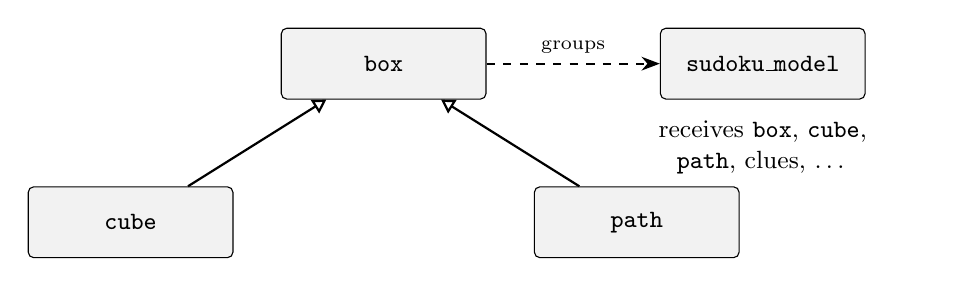
\begin{tikzpicture}[
  cls/.style={draw, rounded corners=2pt, minimum width=2.6cm, minimum height=0.9cm, align=center, font=\small\ttfamily, fill=lightgray},
  arr/.style={-{Triangle[open]}, thick}]
  \node[cls] (box) {box};
  \node[cls, below left=1.1cm and 0.6cm of box] (cube) {cube};
  \node[cls, below right=1.1cm and 0.6cm of box] (path) {path};
  \node[cls, right=2.2cm of box] (model) {sudoku\_model};
  \node[font=\small, below=0.15cm of model, text width=4.2cm, align=center] {receives \texttt{box}, \texttt{cube},\\ \texttt{path}, clues, \ldots};
  \draw[arr] (cube) -- (box);
  \draw[arr] (path) -- (box);
  \draw[-{Stealth}, thick, dashed] (box) -- node[above, font=\scriptsize]{groups} (model);
\end{tikzpicture}
\caption{\texttt{cube} and \texttt{path} are subclasses of \texttt{box}. The model only knows about \texttt{box}.}
\end{figure}

\subsection{\texttt{box}: the generic group (R1)}

The class stores a dictionary $(i,j)\mapsto$ value or \texttt{None} (\texttt{None} is a free cell). It knows nothing about rows, columns or blocks. The parameter \texttt{n} is used only to validate inputs: \texttt{add} raises \texttt{IndexError} for coordinates outside the grid and \texttt{ValueError} for values outside $[1,N]$. Adding a cell that already exists, without a value, does not erase the previous value; two different values for the same cell are rejected.

\begin{lstlisting}
class box:
    def __init__(self, n, cells=None):
        self.n, self.N = n, n * n
        self.cells = {}
        for (i, j), val in (cells or {}).items():
            self.add(i, j, val)

    def add(self, i, j, val=None):
        if not (0 <= i < self.N and 0 <= j < self.N):
            raise IndexError(f"cell ({i},{j}) is outside the grid")
        if val is not None:
            if not (1 <= val <= self.N):
                raise ValueError(f"value {val!r} is outside [1,{self.N}]")
            self.cells[(i, j)] = val
        else:
            self.cells.setdefault((i, j), None)

    def matrix(self):   # zeros in free / non-member cells
        ...
\end{lstlisting}

(Simplified excerpt; the full version, with the type and conflict checks, is in the notebook.)

\subsection{\texttt{cube} and \texttt{path} (R2, R3)}

\texttt{cube(n,i,j)} adds the $n^2$ cells $(i\,n+p,\ j\,n+q)$. \texttt{path(n,start,end)} walks the straight segment between two cells, inclusive, in either direction. With $(i_0,j_0)$ and $(i_1,j_1)$ as the endpoints, the direction is given by the signs of the differences:
\[
  d_i=\mathrm{sgn}(i_1-i_0),\qquad d_j=\mathrm{sgn}(j_1-j_0),
\]
and the cells are $(i_0+t\,d_i,\ j_0+t\,d_j)$ for $t=0..\max(|i_1-i_0|,|j_1-j_0|)$. A segment that is neither horizontal nor vertical is rejected with \texttt{ValueError}.

\begin{lstlisting}
class cube(box):
    def __init__(self, n, i, j):
        super().__init__(n)
        for a in range(n):
            for b in range(n):
                self.add(i * n + a, j * n + b)

class path(box):
    def __init__(self, n, start, end):
        super().__init__(n)
        (i0, j0), (i1, j1) = start, end
        if i0 != i1 and j0 != j1:
            raise ValueError("neither horizontal nor vertical")
        di = (i1 > i0) - (i1 < i0)
        dj = (j1 > j0) - (j1 < j0)
        for t in range(max(abs(i1 - i0), abs(j1 - j0)) + 1):
            self.add(i0 + t * di, j0 + t * dj)
\end{lstlisting}

\subsection{Random clues (R4)}

The function picks $k$ distinct cells at random and pins each to a random value in $[1,N]$, by default with $k=n$. The result is a \texttt{box}, with no new class. The random generator is a parameter, so that tests are reproducible.

\begin{lstlisting}
def random_clues(n, k=None, rng=None):
    rng = rng or random
    N, k = n * n, (n if k is None else k)
    g = box(n)
    all_cells = [(i, j) for i in range(N) for j in range(N)]
    for i, j in rng.sample(all_cells, k):
        g.add(i, j, rng.randint(1, N))
    return g
\end{lstlisting}

\subsection{CSP model and solving (R5)}

The model creates one integer variable in $[1,N]$ per cell. \texttt{add\_groups} accepts an arbitrary number of groups and applies~\eqref{eq:alldiff} and~\eqref{eq:fix}; \texttt{add\_clues} applies only~\eqref{eq:fix}. The method \texttt{solve} returns the grid or \texttt{None}; the attribute \texttt{status} stores the solver status, which makes it possible to tell a puzzle with \emph{no solution} (\texttt{INFEASIBLE}) apart from a \emph{time limit reached} (\texttt{UNKNOWN}).

\begin{lstlisting}
class sudoku_model:
    def __init__(self, n):
        self.n, self.N = n, n * n
        self.m = cp_model.CpModel()
        self.x = [[self.m.NewIntVar(1, self.N, f"x_{i}_{j}")
                   for j in range(self.N)] for i in range(self.N)]

    def add_groups(self, *groups):
        for g in groups:
            if len(g) > 1:
                self.m.AddAllDifferent([self.x[i][j] for (i, j) in g.cells])
            self._pin(g)

    def solve(self, time_limit=None):
        solver = cp_model.CpSolver()
        ...
        st = solver.Solve(self.m)
        self.status = solver.StatusName(st)
        if st in (cp_model.OPTIMAL, cp_model.FEASIBLE):
            return [[solver.Value(v) for v in row] for row in self.x]
        return None
\end{lstlisting}

\subsection{Full Sudoku (R6)}

\texttt{full\_sudoku} joins the $N$ rows (left to right), the $N$ columns (bottom to top, to exercise both directions of \texttt{path}), the $N$ blocks and the clue group. It accepts extra groups, used by the variants in section~\ref{sec:ext}.

Since the clues are random they may be contradictory. The strategy chosen in \texttt{generate\_and\_solve} is to \textbf{re-draw}: generate new clues until the puzzle has a solution (at most 100 attempts) and, if the attempts run out, return \texttt{None}. The justification is in section~\ref{sec:results}.

% =====================================================================
\section{Validation}\label{sec:valid}

Validation is automatic (functions \texttt{validate} and \texttt{run\_tests} in the notebook) and checks:

\begin{itemize}
  \item that every row, column and $n\times n$ block of the solved grid contains exactly $\{1,\dots,N\}$;
  \item that the cells pinned by the clues keep their value in the solution;
  \item that \texttt{add} rejects coordinates outside the grid and values outside $[1,N]$, and that a value neither silently erases nor silently contradicts another;
  \item that \texttt{path} gives the same set of cells in both directions, works with a single point, and rejects diagonals;
  \item that a contradictory puzzle (two values $1$ in the same row) returns \texttt{None} with status \texttt{INFEASIBLE};
  \item the full flow (generate clues $\to$ assemble groups $\to$ solve $\to$ validate) with 20 different seeds for each of $n=2$ and $n=3$.
\end{itemize}

All tests passed. Nothing is hard-wired to $9\times 9$: the same code runs for $n=2$ ($4\times 4$ grid) and up to $n=6$.

% =====================================================================
\section{Results}\label{sec:results}

\subsection{Random puzzles with no solution}

To decide what to do when the random clues are contradictory, we measured the fraction of puzzles with no solution over 200 samples (seeds $0..199$) for several $n$ and $k$.

\begin{table}[h]
\centering
\begin{tabular}{ccc}
\toprule
$n$ & $k$ (number of clues) & Puzzles with no solution \\
\midrule
2 & 2  & 10\,\% \\
2 & 4  & 69\,\% \\
3 & 3  & 8\,\%  \\
3 & 9  & 67\,\% \\
3 & 20 & 98\,\% \\
\bottomrule
\end{tabular}
\caption{Fraction of puzzles with no solution over 200 samples.}
\label{tab:imposs}
\end{table}

With $k=n$ (the default) the fraction is small, so re-drawing the clues almost always converges after one or two attempts. This is the reason for the chosen strategy. As $k$ grows, each new clue may contradict the previous ones and the fraction rises quickly: in that regime re-drawing is no longer a good idea, and it would be better to generate the clues from a complete solution.

\subsection{Scale}

We measured the total time of \texttt{generate\_and\_solve} with $k=n$ clues (seed~1, a single run per value of $n$, wall-clock time).

\begin{table}[h]
\centering
\begin{tabular}{cccc}
\toprule
$n$ & Grid & Time (s) & Attempts \\
\midrule
3 & $9\times 9$   & 0.05  & 1 \\
4 & $16\times 16$ & 0.38  & 1 \\
5 & $25\times 25$ & 2.29  & 1 \\
6 & $36\times 36$ & 10.77 & 1 \\
\bottomrule
\end{tabular}
\caption{Solving time as a function of $n$. All grids were validated.}
\label{tab:scale}
\end{table}

The number of variables grows with $N^2=n^4$ and the number of $\alldiff$ constraints with $3N=3n^2$, each over $N$ variables, so the time grows fast but remains feasible up to $n=6$. These times are for puzzles with very few clues, hence barely constrained: there are many solutions and the solver finds one quickly. We did not measure heavily constrained puzzles, nor repeat each measurement, so the values are indicative only. Re-running the notebook gives slightly different times.

% =====================================================================
\section{Extensions}\label{sec:ext}

In every extension the CSP model stays \textbf{exactly the same}: groups are only added or replaced, which confirms the value of the \texttt{box} abstraction.

\begin{description}[leftmargin=1.5em]
  \item[Diagonal Sudoku (X-Sudoku).] Two \texttt{box}es, one per main diagonal, passed through \texttt{extra}. The solution obtained was also validated on both diagonals.
  \item[Hyper-Sudoku / Windoku.] Four \texttt{box}es with $3\times 3$ blocks with corners $(1,1)$, $(1,5)$, $(5,1)$ and $(5,5)$, overlapping the normal blocks. All four windows of the solution contain $\{1..9\}$.
  \item[Irregular Sudoku (jigsaw).] The regular blocks are replaced by irregular regions, each a \texttt{box} built cell by cell from a letter map. It was tested on a $4\times 4$ grid ($n=2$) with four regions of 4 cells. Note: not every region layout admits a solution; the first layout we tried was impossible even without clues (the solver returned \texttt{INFEASIBLE}) and was replaced by one that has solutions.
  \item[Scale.] See table~\ref{tab:scale}.
\end{description}

The three-dimensional Sudoku extension ($n^2\times n^2\times n^2$) was \textbf{not implemented}.

% =====================================================================
\section{Discussion and limitations}\label{sec:disc}

\paragraph{Design decisions.}
\begin{itemize}
  \item \emph{CP-SAT instead of SCIP:} $\alldiff$ is native and the propagation is specific to this constraint.
  \item \emph{Two methods in the model} (\texttt{add\_groups} and \texttt{add\_clues}), for the reason in section~\ref{sec:clues}. The assignment speaks of one method that imposes ``all different'' and pins the values; following it literally for the clue group would leave most puzzles with no solution.
  \item \emph{Re-drawing clues} when the puzzle is impossible, because it is cheap with small $k$ (table~\ref{tab:imposs}).
  \item \emph{Result} \texttt{None} \emph{plus the attribute} \texttt{status}, to tell ``no solution'' apart from ``time limit reached''.
\end{itemize}

\paragraph{Limitations.}
\begin{itemize}
  \item Random clues do not guarantee a unique solution; the generated puzzle may have many solutions. The solver returns only one.
  \item Validation by sampling (20 seeds per $n$) is not a proof of correctness.
  \item The timing measurements are from a single run and for barely constrained puzzles.
  \item The 3D Sudoku was not done.
\end{itemize}

% =====================================================================
\section{Conclusion}

The \texttt{box} abstraction (a set of cells, some pinned, subject to ``all different'') was enough to represent rows, columns, blocks, random clues and the diagonal, Windoku and jigsaw variants, without changing a line of the CSP model. Solving with CP-SAT is fast for the usual grids and remains feasible up to $36\times 36$ with few clues. Still to do are the three-dimensional extension and a performance analysis with more heavily constrained puzzles.

\end{document}
